\textbf{Ejemplo 13}\\
Suponga que se va a reunir  800.000 COP mediante depósitos mensuales durante 5 años, con la siguiente condición: los depósitos durante el primer año son iguales; para comenzar el segundo año aumentan un 15\% y permanecerán constantes durante ese mismo año: al comenzar el tercer año vuelven a subir otro 15\% y permanecen constantes durante ese año y así sucesivamente.Con una tasa del 27\% efectivo anual: calcular el valor del primer depósito y el valor del último depósito del gradiente escalonado.\\
\\
	%%%%%%%%%%%%%%%%%%% EJERCICIO 13 %%%%%%

%\newpage %USAR SOLO SI EL SOLUCIÓN QUEDA SOLO Y ES NECESARIO BAJARLO A LA SIGUIENTE PAGINA
\textbf{Solución }\\
%La tabla ira centrada
\begin{center}
	\renewcommand{\arraystretch}{1.6}% Margenes de las celdas
	%Creación de la cuadricula de 3 columnas
	\begin{longtable}[H]{|c|c|c|}
		%Creamos una linea horizontal
		\hline
		%Definimos el color de la primera fila
		\rowcolor[HTML]{FFB183}
		%%%%% INICIO ASIGNACIÓN FECHA FOCAL %%%%%%%
		%%%%%%%%%% INICIO TITULO
		%Lo que se hace aquí es mezclar las 3 columnas en una sola
		\multicolumn{3}{|c|}{\cellcolor[HTML]{FFB183}\textbf{1. Asignación período focal}}  \\ \hline
		\multicolumn{3}{|c|}{$pf = \textit{60 pmv}$}   \\\hline
		%%%%%%%%%% FIN TITULO
		%%%%% INICIO DECLARACIÓN DE VARIABLES %%%%%%%
		%%%%%%%%%% INICIO TITULO
		%Lo que se hace aquí es mezclar las 3 columnas en una sola
		\multicolumn{3}{|c|}{\cellcolor[HTML]{FFB183}\textbf{2. Declaración de variables}}   \\ \hline
		%%%%%%%%%% FIN TITULO
		%%%%%%%%%% INICIO DE MATEMÁTICAS
		%Cada & hace referencia al paso de la siguiente columna
		\multicolumn{2}{|c|}{$\hspace{2 cm}VP=  800{.}000COP \hspace{2 cm}$} & $g=15\% \textit{incremento entre depositos anual}$ \\
		\multicolumn{2}{|c|}{$\hspace{2 cm}n_1=5  \textit{ pav} \hspace{2 cm}$} & $i_1=27\% \textit{ pav}$ \\
		\multicolumn{2}{|c|}{$\hspace{2 cm}n_2=12 \textit{ pmv} \hspace{2 cm}$} & $i_2=?\% \textit{ pmv}$ \\ 
		\multicolumn{2}{|c|}{$\hspace{2 cm}R_{1}= ?COP  \textit{} \hspace{2 cm}$} & $R_{60}= ?COP  \textit{ }$ \\\hline	
		
		%%%%%%%%%% FIN DE MATEMÁTICAS
		%%%%% FIN DECLARACIÓN DE VARIABLES
		
		%%%%% INICIO FLUJO DE CAJA
		\rowcolor[HTML]{FFB183}
		\multicolumn{3}{|c|}{\cellcolor[HTML]{FFB183}\textbf{3. Diagrama de flujo de caja}} \\ \hline
		%Mezclamos 3 columnas y pondremos el dibujo
		%%%%%%%%%%%%% INSERCIÓN DE LA IMAGEN
		%Deberán descargar las imágenes respectivas del drive y pegarlas en la carpeta
		%n_capitulo/img/ejemplos/1/capitulo1ejemplo1.pdf  (el /1/ es el numero del ejemplo)
		\multicolumn{3}{|c|}{ 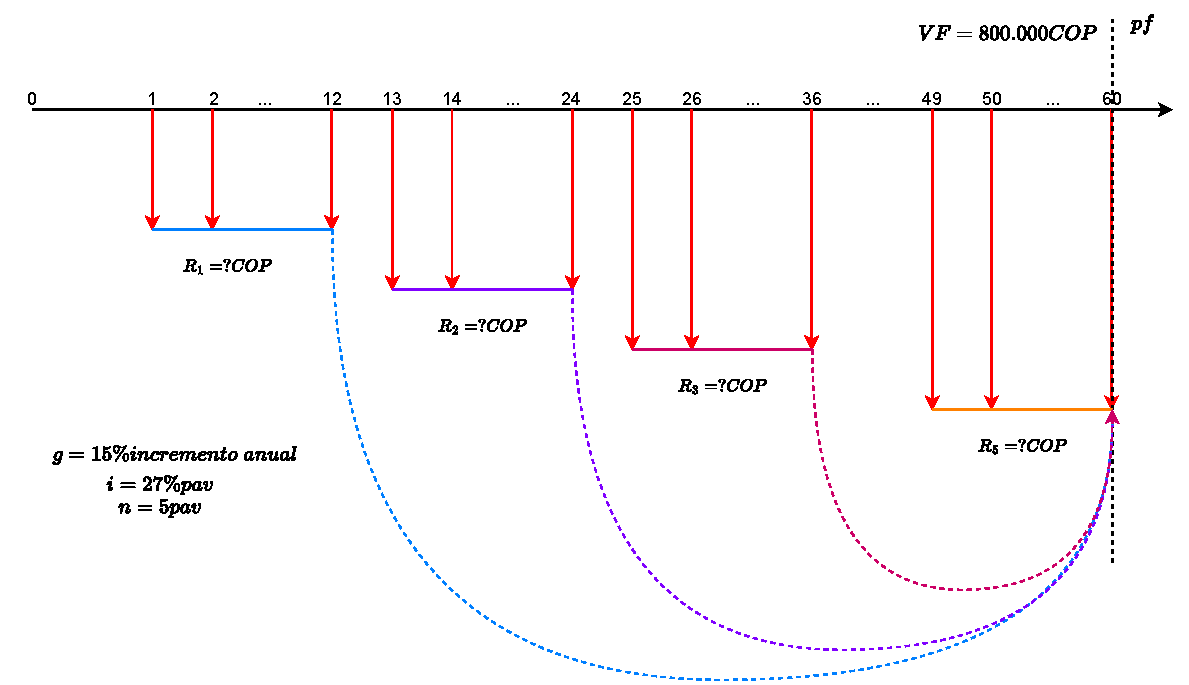
\includegraphics[trim=-5 -5 -5 -5 , scale=0.6]{6_Capitulo/img/ejemplos/13/Capitulo6Ejemplo13.pdf} }
		\\ \hline
		%%%%%%%%%%%%% FIN INSERCIÓN DE IMAGEN
		%%%%%FIN FLUJO DE CAJA
		
		%%%%% INICIO DECLARACIÓN FORMULAS
		%%%%%%%%%%% INICIO TITULO
		\rowcolor[HTML]{FFB183}
		\multicolumn{3}{|c|}{\cellcolor[HTML]{FFB183}\textbf{4. Declaración de fórmulas}}    \\ \hline
		%%%%%%%%%%% FIN TITULO
		%%%%%%%%%%% INICIO MATEMÁTICAS
		\multicolumn{3}{|c|}{$(1+i_1)^{m1} \equiv (1+i_2)^{m2} \hspace{0.4 cm} \textit{ Equivalencia de tasas }$} \\
		\multicolumn{3}{|c|}{$VF=\frac{(R)[(1+i)^{n}(1+i)^{-n}]}{g-i} \hspace{0.4 cm} \textit{Valor futuro de un gradiente aritmético si } g \neq i $} \\  
		\multicolumn{3}{|c|}{$R_n=R_{n-1}(1+g)^{n-1} \hspace{0.4 cm} \textit{Valor del flujo de n gradiente geométrico}$} \\ 
		\multicolumn{3}{|c|}{$VF=\frac{R(1+i)^{n}-i}{i} \hspace{0.4 cm} \textit{Valor futuro de una serie uniforme } $} \\\hline
		
		%%%%%%%%%% FIN MATEMÁTICAS
		%%%%%% INICIO DESARROLLO MATEMÁTICO
		\rowcolor[HTML]{FFB183}
		%%%%%%%%%%INICIO TITULO
		\multicolumn{3}{|c|}{\cellcolor[HTML]{FFB183}\textbf{5. Desarrollo matemático}}       \\ \hline
		%%%%%%%%%% FIN TITULO
		%%%%%%%%%% INICIO MATEMÁTICAS
		\multicolumn{3}{|c|}{$(1+0.27)^{1} \equiv (1+i_2)^{12}$} \\
		\multicolumn{3}{|c|}{\textit{Despejando se obtiene: } }\\
		\multicolumn{3}{|c|}{$(1.27)^{0.5}-1 \equiv i_2 \hspace{0.2 cm}\rightarrow \hspace{0.2 cm} i_2=2.01178\% \textit{ pmv} $} \\
		\multicolumn{3}{|c|}{\textit{Primero comenzamos los cálculos con el gradiente simple y hallamos el valor de la cuotas $R_1$ } }\\
		\multicolumn{3}{|c|}{$  800{.}000COP=\frac{(R)(1.14)^{5}-(1.27)^{5}}{0.15-0.27}$} \\
		\multicolumn{3}{|c|}{\textit{Donde se obtiene: }$R_1=   74{.}275.83COP$} \\
		\multicolumn{3}{|c|}{$R_5=74{.}275.83COP*(1.15)^4=129{.}908.88 COP$}\\
		\multicolumn{3}{|c|}{\textit{Utilizando la fórmula del valor futuro de una serie uniforme se procede a calcular $R_1$ y $R_{60}$} }\\
		\multicolumn{3}{|c|}{$  74{.}275.83COP=\frac{(R_1)((1.02)^{12}-1)}{0.02} \hspace{0.2 cm}\rightarrow \hspace{0.2 cm} R_1=  5{.}537.97COP$} \\
		 \multicolumn{3}{|c|}{\textit{De igual forma la última cuota se podra calcular así:  } }\\
		 \multicolumn{3}{|c|}{$  129{.}908.88COP=\frac{(R_{60})((1.02)^{12}-1)}{0.02} \hspace{0.2 cm}\rightarrow \hspace{0.2 cm} R_{60}=  9{.}658.95COP$} \\\hline
		%%%%%%%%%% FIN MATEMÁTICAS
		%%%%%% FIN DESARROLLO MATEMÁTICO
		%%%%%% INICIO RESPUESTA
		\rowcolor[HTML]{FFB183}
		%%%%%%%%%%INICIO TITULO
		\multicolumn{3}{|c|}{\cellcolor[HTML]{FFB183}\textbf{6. Respuesta}}   \\ \hline
		%%%%%%%%%% FIN TITULO
		%%%%%%%%%% INICIO RESPUESTA MATEMÁTICA
		\multicolumn{3}{|c|}{${ R_{60}=  9{.}658.95COP }$} \\
		\multicolumn{3}{|c|}{${R_1=  5{.}537.97 COP}$} \\\hline
		%%%%%%%%%% FIN MATEMÁTICAS
		%%%%%% FIN RESPUESTA
	\end{longtable}
	%Se crean dos lineas en blanco para que no quede el siguiente texto tan pegado
	%\newline \newline %USARLO SI CREES QUE ES NECESARIO
\end{center}

%%%%%%%%%%%%%%%%%%%%%%%%%%FIN EJERCICIO 13 %%%%%%%%%%%%%%%%%%%%%%%%%%%

